
%% bare_adv.tex
%% V1.4b
%% 2015/08/26
%% by Michael Shell
%% See:
%% http://www.michaelshell.org/
%% for current contact information.
%%
%% This is a skeleton file demonstrating the advanced use of IEEEtran.cls
%% (requires IEEEtran.cls version 1.8b or later) with an IEEE Computer
%% Society journal paper.
%%
%% Support sites:
%% http://www.michaelshell.org/tex/ieeetran/
%% http://www.ctan.org/pkg/ieeetran
%% and


%
\documentclass[10pt,journal,compsoc]{IEEEtran}


\usepackage{cite}
\usepackage[pdftex]{graphicx}
\usepackage{amsmath}
\usepackage{algorithmic}
\usepackage{array}
\usepackage[caption=false,font=footnotesize]{subfig}
\usepackage{url}
\usepackage{caption}%add thi sentence can centering the caption.
\usepackage{multirow}% creat multirow table need to the packet
\usepackage{booktabs}% three table creating need to the packet
\usepackage{amssymb }% insert cuntermark
\usepackage{indentfirst}%��1.5���ַ�
\usepackage{ragged2e}
%\usepackage{mathtools}
\usepackage{amsmath}

\hyphenation{op-tical net-works semi-conduc-tor}
\makeatletter
\newcommand{\rmnum}[1]{\romannumeral #1}
\newcommand{\Rmnum}[1]{\expandafter\@slowromancap\romannumeral #1@}
\usepackage{bm}
\makeatother

\begin{document}
%
% paper title
% Titles are generally capitalized except for words such as a, an, and, as,
% at, but, by, for, in, nor, of, on, or, the, to and up, which are usually
% not capitalized unless they are the first or last word of the title.
% Linebreaks \\ can be used within to get better formatting as desired.
% Do not put math or special symbols in the title.
\title{A Survey on Motion Detecting Techniques and Influence using WiFi Signal}


\author{Lei~Wang,~\IEEEmembership{Member,~IEEE,}
        Linlin~Guo, Jialin Liu and ~Wei~Zhou}
\renewcommand{\raggedright}{\leftskip=0pt \rightskip=0pt plus 0cm}
\IEEEtitleabstractindextext{%
\begin{abstract}
\raggedright
Some applications using WiFi signal have been increasing attention and studied for the past 2 decades such as Indoor location, human activity recognition, health monitoring and access control. According to the characteristic of WiFi signal, it is sensitive to the environment change.Development of those applications encounter challenge which are indoor environment change, device diversity and motion influence and so on. this article mainly addresses the problem of motion influence reflected by WiFi signals. Due to the fact that There are different affection on WiFi signal based these application. we survey influence of motion from these application and develop trend of WiFi signals. Specifically, we first study the WiFi signal information which are used these applications: such as RSS, CSI, AOA and TOF. Next, we summary challenges and problems from WiFi signal based application in order to improve the accuracy of these application. Moreover, we show how to deal with the influence of motion in wireless network for these applications. then, we discuss that pay closed attention to opportunities and future research directions in this new and largely open area.
\end{abstract}

% Note that keywords are not normally used for peerreview papers.
\begin{IEEEkeywords}
Motion Detecting, Indoor Location , Wireless Signals ,Physical Layer Information.
\end{IEEEkeywords}}


% make the title area
\maketitle

%\IEEEdisplaynontitleabstractindextext
% \IEEEdisplaynontitleabstractindextext has no effect when using
% compsoc under a non-conference mode.

\IEEEpeerreviewmaketitle


\ifCLASSOPTIONcompsoc
\IEEEraisesectionheading{\section{Introduction}\label{sec:introduction}}
\else
\section{Introduction}
\label{sec:introduction}
\fi

\IEEEPARstart{D}{URING} the past decade, there has been an exceptional development of wireless network and mobile device such as WiFi signal or smart phone. WiFi signals are typically information carriers between a transmitter and a receiver. WiFi can also extend our senses, enabling us to see moving objects through walls and behind closed doors. This view apply to security surveillance and saving hostages in current wireless network world. Of course, we also can recognize fine-grained gesture activity made behind a wall, such as push, pull and so on.

Providing accurate and opportune information on people's location, human activities and behaviors is one of the most important tasks in pervasive computing.With the development and popularization of Wi-Fi, surfing on Internet with mobile devices has become an indispensable of people's daily life. Human body is a strong electromagnetic energy absorption object, which may cause directional shadowing effect to wireless signal. Therefore, when the same device is placed at different position near human body, e.g. Shirt pocket or back pocket, the RSS measurement will be obviously deviated.

Providing accurate and opportune information on people's location, human activities and behaviors is one of the most important tasks in pervasive computing.Activity recognition means that leverage PHY layer information to indicate the human activities in indoor environment and then learn the specific pattern related with a specific human activity\cite{14}\cite{17}.

\textbf{Introduce mobility} Mobility information, as a new dimension in addition to wireless signals, can benefit localization in a number of ways, since location and mobility are by nature related in the physical world


\textbf{Indoor Location}:\cite{5},\cite{13},\cite{19},\cite{20},\cite{21},\cite{22},\cite{23},\cite{24},\cite{26},\cite{27},
\cite{28},\cite{29},\cite{35},\cite{49},\cite{54},\cite{55},\cite{56},\cite{70},\cite{72},\cite{73},\cite{74},\cite{75}.

\textbf{Human Activity Recognition}:\cite{2},\cite{6},\cite{9},\cite{10},\cite{11},\cite{14},\cite{15},\cite{16},
\cite{17},\cite{18},\cite{37},\cite{42},\cite{43},\cite{44},\cite{45},\cite{46},\cite{47}.

\textbf{Access Control and User Authentication}:\cite{41},\cite{3},\cite{4},\cite{6},\cite{7},\cite{31},\cite{32},\cite{34},\cite{36},\cite{39}

\textbf{Keyword Recognition}:\cite{63},\cite{64},\cite{66}

\textbf{Detecting Mobility}:\cite{1},\cite{9},\cite{10},\cite{18},\cite{37},\cite{50},\cite{51},\cite{52},\cite{53},\cite{57},\cite{59},\cite{60},\cite{61},\cite{62}
,\cite{68},\cite{69},\cite{70},\cite{71},\cite{72},\cite{73}

\textbf{WiFi Signal Information and knowledge}:\cite{40},\cite{8},\cite{12},\cite{48},\cite{58},





\text{outline}:
\begin{itemize}

\item Introduction
\item WiFi signal Information and Technical
\item Challenge and issue
\item How to deal with error from motion influence for WiFi signal based application
\item Discuss future research direction
\item Conclusion

\end{itemize}

%\hfill mds

%\hfill August 26, 2015

\subsection{Background Significance}
Location is playing an ever increasing role in mobile computing. Many of the most popular applications and services used today build on knowing the user's current location. For many of these applications the accuracy of current technologies is adequate. However, we believe the next generation of mobile applications and services will need to a next generation location technology that provide accurate, reliable location information for indoor environments. We discussed how it has been designed and developed to provide application and service developers easy access to indoor location information. More broadly, we believe efficient and accurate room level location can open many new application opportunities.

In the static environmen t, motion influence come from two factor that environment changes and human motion; self-motion of objector has a important role in the influence of motion��In generally, some work neglect this factor due to this influence of self-motion was treated as least factor. However, according to experiment we show that self-motion influence has a important effective on micro-motion detection in some proposes works.
\begin{figure}[hbt]
\centering
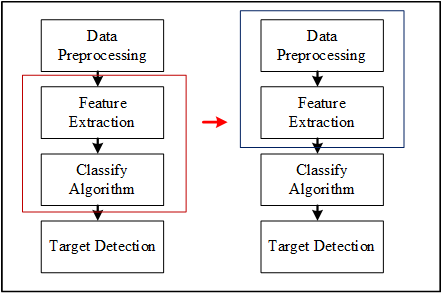
\includegraphics[width=2.5in]{fig/framework.png}
\caption{Design framework}
\label{fig flow}
\end{figure}


\subsection{Challenges and Issues}

\textbf{Los and NLoS}: According to the NLOS/LOS conditions, PHY layer setings

In general,Noise oftern are classified as following three part:
1) The first type of noise is the slight RSS fluctuation due to environment Gaussian noise.
2)The second type of noise is caused by small environment changes such as device perturbation in one's hand or people walking nearby.
3) Exists some impulsive noise in the RSS sequence for some type of mobile phones.
\cite{8}\cite{84}

 text here.
\begin{figure}[hbt]
\centering
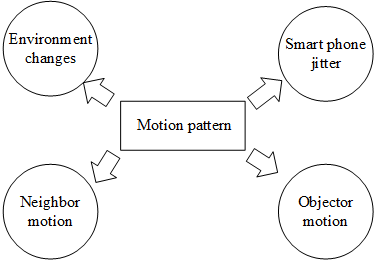
\includegraphics[width=2.0in]{fig/motion.png}
\caption{Motion Pattern}
\label{fig flow}
\end{figure}
\begin{figure}[hbt]
\centering
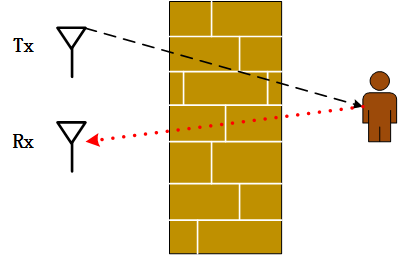
\includegraphics[width=2.0in]{fig/throughwall.png}
\caption{see through wall using WiFi signal}
\label{fig flow}
\end{figure}

In this article, we survey this new trend of mobility enhancing human computing using WiFi signals. Specifically, we first study how to WiFi signals measures: what types of wifi measures we can use and what types of mobility information we can acquire. Next, we discuss how mobility influent wifi signals on different application in wireless networks.by introducing some application of wifi signals, acquire the accuracy influence of motion in wireless networks. mobility offer enhancing localization accuracy, decreasing deployment cost and enriching location context.
Combining existing work and our own working experiences, we emphasize the principles and conduct a comparative study of the mainstream technologies. Finally, we conclude this survey by addressing future research directions and opportunities in this new and largely open area.

\subsection{Contribution}

Our main contribution are summarized as follows
\begin{itemize}

\item To the best of our knowledge, this is survey about mobility influence of practical application based on WiFi signals(this is survey on application based on WiFi signals from the mobility influence).the above mentioned application based on WiFi signals contain indoor localization, human activity, target tracking and access control in wireless network.

\item We list the different mobility patterns of those application and the corresponding challenges, as well as provide a comprehensive comparison for each category application in the term of accuracy, metric, device and cost and so on.

\item We provide that new solutions for the above mention challenge.

\item Finally, we discuss the open research issues.

\end{itemize}

\section{Motion types and Measuring Principles}
\subsection{Introduction of Related Technical Method}
wireless radio propagation in compact environment could be modeled as a superposition of large-scale path-loss, middle-scale shadowing, and small-scale multipath fading\cite{48}. A wireless signal traverses in all radial directions, and reflects off walls, furniture, and other objects. Due to reflections, multiple copies of the same signal arrives at the receiver, each undergoing different delay and attenuation - a phenomena which is commonly called multipath. Definition of the direct path is the straight line joining the transmitter and the receiver. A wireless signal is composed of a direct path, and other reflected components, and suffers attenuation as it propagates from the transmitter to the receiver. Indoors, wireless attenuation is mainly caused by path-loss, and multipath reflections.
The main Information measurements of WiFi signals are summarized as follows:\\
\begin{itemize}
\item \textbf{RSS}\\
The wireless channel between the client and the AP is expected to vary under environmental or device mobility. This is because the fine-grained multipath structure may change if there are moving objects in the environment, or the device itself moves. These fine-grained variations of the wireless channel can not be captured by RSSI because it only captures an aggregate indicator of all the multipath components.

It is possible to estimate a crude distance between the transmitter and the receiver by using the received energy at the receiver$(P_{R})$ in the path-loss equation:
\begin{equation}\label{1}
  P_{R}=P_{0}-10\gamma log{(d)}
\end{equation}
where $P_{0}$ is the received energy at a distance of 1m from the transmitter,$d$ is the distance between the transmitter, and the recevier in meters; and $\gamma$ is the path loss exponent. $\gamma$ depends on the propagation characteristics of the received signal. Earlier approaches have typically used RSSI as the received energy$(P_{R})$ in the above path loss equation\cite{12}. However, RSSI is an union of the energy of all the signal paths-direct as well as multipath reflections. If we use RSSI as $P_{R}$, we will need to estimate the propagation characteristics of all the signal paths, to correctly choose the path-loss exponent. Unfortunately, today's WiFi cards do not expose any specific multipath information, making it difficult to model the aggregate signal(RSSI), we show that it is easier to only use the energy of the reflected paths, it can be a robust indicator of distance, even in dynamic indoor environments.
\item \textbf{CSI}\\
CSI is not a simple extension of RSS on physical subcarrier but it reveals totally different information on frequency selective fading process. The CSI is reported as a matrix of complex numbers representing the channel gain for every subcarrier and for every transmit-receive antenna pair. By an appropriate Inverse Fast Transformation (IFFT), the frequency-domain CSI can be translated into the time-domain power-delay profile (PDP). PDP captures the energy of the different paths incident at increasing delays. Since, the direct path traverses the minimum distance amongst all the received paths, its energy will likely appear in the earliest component of the PDP.
\item \textbf{TOF}\\
Systems that use timestamps reported by WiFi cards can obtain time of flight at a granularity of several nanoseconds, requiring in ranging error of few meters.Means the time it takes for its signal to travel from its transmit antenna to the reflecting body, and then back to each of its receive antennas. WiTrack obtains an initial measurement of the TOF using FMCW transmission technique; it then cleans this estimate to eliminate multipath effects and abrupt jumps due to noise.FMCW transmits a narrowband signal whose carrier frequency changes linearly with time. To identify the distance from a reflector, FMCW compares the carrier frequency of the reflected signal to that of the transmitted signal. Since the carrier frequency is changing linearly in time, delays in the reflected signals translate into frequency shifts in comparison to the transmitted wave.

Specifically, we know from basic electromagnetics that as a signal propagates in time, it accumulates a corresponding phase depending o its frequency. The higher the frequency of the signal, the faster the phase accumulates. To illustrate, let us consider a transmitter sending a signal to its receiver. Then we can write the wireless channel $h$ as :
\begin{equation}\label{5}
h=ae^{-j2\pi f\tau }
\end{equation}

where $a$ is the signal magnitude, $f$ is the frequency and $\tau$ is the time-of-flight. The phase of this channel depends on time-of-flight as:
\begin{equation}\label{6}
  \angle h=-2\pi f \tau mod 2\pi
\end{equation}
Notice that the above equation depends directly on the signal's time-of-flight and hence, we can use it to measure the time-of-flight $\tau$ as
\begin{equation}\label{7}
 \tau =-\frac{\angle h}{2\pi f} mod \frac{1}{f}
\end{equation}
The above equation gives us the time-of-flight modulo $1/f$. Hence, for a wifi frequency of 2.4 GHz, we can only obtain the time-of-flight modulo 0.4 nanoseconds.
\item \textbf{AOA}\\
In general, we leverage AOA information to locate target in indoor environment. how to get AOA information from wireless network by the smart phone or other mobile device.  MUSIC algorithm can get AOA information. AOA means wireless signals of arrive of angle from transmitter to receiver. Moreover, AOA treat as add dimension information to locate target for improving accuracy of location. the key point need to get transmitter location information,then by MUSIC\cite{49} algorithm computing AOA information, next leverage triangle relation to locate target. AOA measures [-90,90] in antenna array.  
A wireless transmission from the client arrives at several angles at the AP. If we can determine the angle of the direct path or ANDP. It is possible to combine the angle of the client with her distance, ultimately yielding her location. Existing AOA estimation algorithms analyze the received signal on multiple antennas to find out the angular components of the signal\cite{81}. The key idea is to analyze the phase of the received signal, a quantity which changes linearly by 2$\pi$ for every wavelength$(\lambda)$ traversed by the signal. For the simplicity of explanation, consider s single path between the transmitter and the receiver. Let us consider that the AP has only two antennas, placed at a distance of $\frac{\lambda}{2}$. Let $\theta$ be the angle at which the signal arrives at the two antennas. The signal travels an extra distance before reaching the second (left) antenna. This extra distance$(\Delta)$ can be approximated as:
\begin{equation}\label{2}
  \Delta d=\frac{\lambda }{2}sin(\theta )
\end{equation}

We know that an extra distance $\Delta d$ will result into a phase difference $(\Delta \phi)$:\\
\begin{equation}\label{3}
 \Delta \phi =\frac{2\pi \Delta d}{\lambda }
\end{equation}

Thus, by observing the phase difference$(\Delta \phi)$ of the arriving signal, we can find the angle-of-arrival as:\\
\begin{equation}\label{4}
  \theta =arcsin( \frac{\Delta \phi}{\pi})
\end{equation}

The above explanation assumes that the arriving signal has only one angular component. In reality, a wireless signal will propagate through multiple paths. AoA estimation algorithm can identify the angles of multiple paths by using many antennas.


With the proliferation of WiFi APs with multiple antennas to support MIMO communications, antenna array based techniques which use multiple antennas at the AP have gained interest recently. The basic idea of these systems is to calculate the AoAs of the multiple signals received at each AP, find the AoA of the direct path to the target, and then apply triangulation to localize\cite{76}\cite{20}\cite{77}\cite{78}\cite{79}.

\begin{table}[htbp]
\center
\scriptsize
\caption{\label{tab:test}WiFi Signal Information in indoor location}
\begin{tabular}{cp{1cm}cp{1cm}p{1cm}}
\toprule
Information & Accuracy & Device & Adaptation & Complexity \\
\midrule
RSS& 2 m & common device  &  low & low\\
CSI& 1 m &5300 or athros or usrp & middle & middle\\
AOA& 1 m & antennas  & high & middle\\
TOF& 60 cm& specific device & high & high\\
\bottomrule
\end{tabular}
\end{table}

Different WiFi signal information provide different accuracy in table 1. Accuracy of indoor location has most high accuracy using TOF, then AOA, RSS is the worst. But, RSS information for common device is feasible. Table 1 show that the accuracy means average accuracy in above applications.

\begin{table}[htbp]
\center
\scriptsize
\caption{\label{tab:test}RF Attenuation in Common Building Materials at 2.4GHz\cite{80}}
\begin{tabular}{cc}
\toprule
 Building Materials & 2.4 GHz \\
\midrule
Glass & 3 dB \\
Solid Wood Door 1.75inches & 6 dB \\
Interior Hollow Wall 6 inches & 6 dB \\
Concrete Wall 18 inches & 18 dB\\
Reinforced Concrete & 40 dB\\
Brick 3.5 inches & 6dB\\
Steel Fire and  Exit Door 2.5 inches& 19 dB\\

\bottomrule
\end{tabular}
\end{table}


\end{itemize}
\begin{table}[htbp]
\center
\scriptsize
\caption{\label{tab:test}summary of application using wifi signals}
\begin{tabular}{ccccc}
\toprule
 Citation & RSS & CSI & AOA & TOF \\
\midrule
RADAR\cite{21} & \checkmark & & &  \\
Horus\cite{27} & \checkmark &  & &  \\
Zee\cite{19} &  & \checkmark & &   \\
SpinLoc\cite{35} & & \checkmark & &  \\
CLAC\cite{4} & \checkmark & \checkmark & &  \\
Arraytrack & & & \checkmark &  \\
Ubicarse\cite{20} &  &  & \checkmark  &   \\
SpotFicite\cite{49} & & & \checkmark & \checkmark \\
Chronos\cite{5} & & & &\checkmark \\
\bottomrule
\end{tabular}
\end{table}

\textbf{Non-invasive human detect}: Wireless non-invasive human detection systems detect and localize humans via their impact on received signal, while the targets carry no wireless-enabled devices.

\textbf{Device-free passive motion detect}: seeks to monitor whether there are people moving in an are of interest-- the detected individual neither carrying any device nor actively participating in the detection progress.


%SpinLoc\cite{35}
On observing that the statistical spectral structures of small-scale multipath signals possess resistance to irrelevant background dynamics while retaining sensitivity to nearby human locomotion. We propose to leverage the histogram feature of the subcarrier amplitudes as signatures for our omnidirectional passive human detection


\textbf{Locate a number of human solutions}: In order to address the non-linearity of the impact of multiple subjects, we propose a successive cancellation based algorithm to iteratively determine the number of subjects. We model indoor human trajectories as a state transition process, exploit indoor human mobility constraints and integrate all information into a conditional random field (CFR) to simultaneously localize multiple subjects, \textbf{SCPL: Indoor Device-free multi-subject counting and localization using radio signal strength}

\textbf{Indoor Localization}: Indoor localization systems using WiFi infrastructure should ideally satisfy the following three requirements.
\begin{itemize}
\item \textbf{Deployable}: They should be easily deployable on existing commodity WiFi infrastructure without requiring any hardware of firmware changes at the access points(APs); they should only work with information like RSS and CSI that is already exposed by commodity, deployed APs.
\item \textbf{Universal}: They should b e able to localize any target device that has a commodity WiFi chip and nothing else. They should not require the target to have any other hardware, be it sensors such as accelerometers, gyroscopes, barometers, cameras, etc., or radios such as UWB, ultrasound, Bluetooth LE, etc.
\item \textbf{Accurate}: They should be accurate, ideally as accurate as the best known localization systems that use wireless signals(even including those that do not satisfy the above two requirements). To the best of our knowledge, the most accurate such localization systems are ArrayTrack \cite{76}and Ubicarse\cite{20} and these systems achieve an accuracy ranging from 30-50 cm in office environments. Achieveing such accuracy would be the target.
\end{itemize}

\textbf{Detecting different motions}: The wireless channel between the client and the AP is expected to vary under environmental or device mobility. This is because the fine-grained multipath structure may change if there are moving objects in the environment, or the device itself moves. These fine-grained variations of the wireless channel can not be captured by RSSI because it only captures an aggregate indicator of all the multipath components.On \cite{60}observing that the statistical spectral structures of small-scale multipath signals possess resistance to irrelevant background dynamics while retaining sensitivity to nearby human locomotion. We propose to leverage the histogram feature of the subcarrier amplitudes as signatures for our omnidirectional passive human detection

\textbf{Tracking user behavior}: In the air user interfaces can be divide into two classes. The first class is based on defining a limited set of gestures and using machine learning to learn patterns and classify gestures into the learned categories. The second class includes interfaces enabled by systems such as RF-IDRAW and WiDraw.These interfaces require no priori learning and can track an arbitrary set of hand motions,enabling a much richer set of applications.Note that only mobility information in employed but no Wi-Fi measurements are required during this trajectory embedding process. To eventually generate a fingerprint database, however, zee still expects users to record Wi-Fi measurements during their moving paths, which will then be annotated with the locations estimated from trajectory embedding

\subsection{Motion Types}
In general, WiFi signals are sensitive to indoor environment changes which contain different influence from different motion type in the indoor environment. It is common hard questions for most researchers to proposed a effective methods adapting dynamic complexity environment. Of course, this questions are challenges. In every research work, authors often show that exists challenges and hard in their work. Motion influence play a important role in wireless network. Goal of this paper mains analysis influence of mobility  for WiFi signal, and try to find a adaptive solutions which estimate mobility influence in different scenarios using fit metric. If so that, mobility factor treat as addition dimension to improving WiFi signal sensing accuracy in complexity indoor environment.

Motion types dived into three classes. The first, target mobility has important influence on WiFi signal is common phenomenon in practical daily life for people. For example, target often walk in public workhouse. Second, surround object mobility result in WiFi signals change to affect target identify. This part is most important challenge for current wireless environment application. For example, Indoor location systems in recent often face with non-target interference. It is hard to identify target and non-target using WiFi signals if target and non-target without attach devices stay static in indoor environment. Similar problems have occurred, non-target mobility have un-neglectable influence to  localizing target. Specifically, CSI (Channel Static Information) has high sensitive to surround environment changes, even small change may product important influence. So, non-target mobility influence for WiFi signal is key point to solute high location problem.

\textbf{Target Mobility}: Target mobility need to face some challenges. Static target is not often occur in practical daily, moving state is common behavior due to human activity. So, we proposed some methods or systems to solute Target mobility such as detecting moving target or locating mobility target and so on. what dose occurs in target mobility? It can change distance of target from transmitter to receiver, enrich multipath effec, add environment complexity. the classic method leverages los identify to locate target or detect moving target\cite{10}.
\begin{figure}[hbt]
\centering
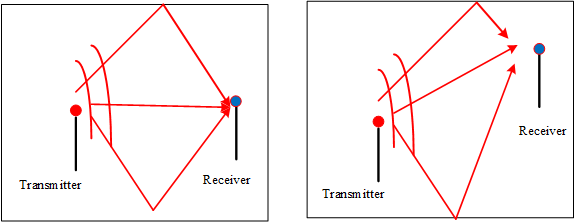
\includegraphics[width=3.0in]{fig/targetmove.png}
\caption{Change of the target moving}
\label{fig flow}
\end{figure}

\textbf{Non-target Mobility}: Non-target mobility means other move object which are normal daily in public workplace such as laboratory or office. Next, Non-target mobility bring a complexity computing of WiFi signals influence in wireless networks. Sometime, Non-target mobility reflected by WiFi signal more than high target.In this event, how to distinguish  mobility influence of target from non-target is essential and important for application which depend on WiFi signals change.

\textbf{Indoor Environment Changes}: Indoor environment changes contains several aspects in the practical environment. In this paper, we give a specially definition of indoor environment from two aspects. One is that add some things to indoor or remove some things. Second is that rearrange the furniture in the indoor. In simple speaking, we only explain simple cases in our daily. Indoor environment changes only impact the multi-path effect.

\textbf{Wireless Device Jitter}: Target with handhold mobile device is hard to keep balance state in motion scenarios. Mobile device jitter result from arm movement of target can cause  small changes of WiFi signal. Just so, this small change is hard different from change of WiFi signal from target self moving.



\subsection{Measuring Principals and Motion Information}
\textbf{Equipment Requirement}:1) The CSI tool is built on the Intel Wi-Fi Wireless Link 5300 802.11n MIMO radios, using custom modified firmware and open source Linux wireless drivers. The IWL5300 provide 802.11n channel state information in a format that reports the channel matrices for 30 subcarrier groups, which is about one group for every 2 subcarriers at 20HMz or one in 4 at 40HMz.\\
2) Atheros CSI Tool


\section{Performance and Metrics}
RADAR \cite{21} operates by recording and processing signal strength information at multiple base stations positioned to provide overlapping coverage in the area of interest.  It combines empirical measurements with signal propagation modeling to determine user location and thereby enable location aware services and application.

Zee\cite{19} Notes that only mobility information in employed but no Wi-Fi measurements are required during this trajectory embedding process. To eventually generate a fingerprint database, however, zee still expects users to record Wi-Fi measurements during their moving paths, which will then be annotated with the locations estimated from trajectory embedding.

\textbf{Fingerprint based }: In indoor environment, fingerprint based methods, first collect fingerprint of Wi-Fi signal in advance at known locations inside a building, and then identify the user��s location by matching the fingerprint of this user with the fingerprint stored in database.Wi-Fi fingerprint-based schemes can provide meter-level indoor localization accuracy at the expense of explicit site-survey (its high deployment cost and low adaptiveness to environment change hinders the practical effectiveness)\cite{74}.

1) Among these approaches, a hot research trend is to incorporate crowd-souring model and built-in sensors in today��s smart-phone.

2) We believe there are plenty of room for improving the localization accuracy while reducing or even eliminating the dependence of site-survey and noisy inertial sensors.

3) It has been widely known that the RSS value is affected by many factors, e.g., the RSS values collected at the same location using same devices with same Wi-Fi APs could fluctuate to a few db depending on how users hold and block the signal

\textbf{Crowdsourcing based}: Crowdsourcing based method leverages large mobile devices which are spread over users to collect data information from existing surround environment. It reduce cost of people, financial resources by using crowdsourced. However, crowdosourcing based method has some challenges in the practical environment. First, Data information collected by crowdsouring is not sure safety and high quality due to identify of mobile device is stranger. Second,  location distribution of collecting information is uneven. If so that, Collecting information can not represent global state of indoor environment. Third, diversity of different mobile device bring small difference to enhanced the inaccuracy data information\cite{22}. In summary, Goal of Crowdsourcing based get high accuracy and low computaitonal requirements.

\textbf{Probability Model based}: Probability model based methods occurred in the previous work.  Probability model construct by training  collected information. However, probability model based method is not pervasive for different environment. this model has not invalidation when environment occurs change\cite{27}. Radio-map based techniques can be categorize into two broad categories: deterministic techniques and probabilistic techniques. Deterministic techniques represent the signal strength of an access point at a location by a scalar value, for example, the mean value, and use non-probabilistic approaches to estimate the user location. On the other hand, probabilistic techniques store information about signal stength distributions from the access point in the radio map and use probabilistic techniques to estimate the user location.

\section{How to deal with Motion Influence}

\subsection{advantage}
understanding patterns of human indoor movement can be valuable in identifying hot spots and corridors that help energy management and commercial site selection. Dfp provides a non-intrusive and private solution to capturing indoor locations.



WiGest\cite{47} showed that as long as the interfering user is more than 4ft away, she has no-effect on accuracy. However, a close-by user by less than 3ft reduces accuracy of the gesture recognition.


\subsection{disadvantage}





\section{Discussion and Future Directions}
\subsection{Discussion}

\textbf{AP Location}:
the placement of AP will impacts the accuracy of the recognition system. In particular, the floor is not the best loation to recognition human activity.\\
\textbf{Device diversity}:
Device diversity also is factor which affect WiFi signal changes in public workplace. In this paper, Device diversity only means different device  discrepancy. In previous works, device diversity do not get more attention for application using WiFi signals. Further, this fine-grained details are neglected by changes of coarse granularity WiFi signals. NiFi system proposed identify user method by  using sequence similar of WiFi signals, meantime device diversity also are consider\cite{6}. Different phones may have different transmission power, antenna layout and hardware configuration. NiFi proposed a shift-cancellation approach to mitigate the impact of device diversity.\\
\textbf{Numbers of Antennas}:\\ Linear antennas offered by commodity WiFi hardware contain three in our daily. Of course, in order to get high accuracy and high resolution may contain more antennas, but this condition need to design according to different application. Array-Track system \cite{76}need 16 antennas to construct rectangular array which can compute AoA for high localization accuracy, or need 8 antennas of \cite{82},\cite{83}. Even the few recent proposals to localize using one WiFi access point require users to walk to multiple locations to emulate the presence of multiple access point.  They then intersect signal measurements across these location coupled with accelerometer readings to infer the user's trajectory.

\textbf{Indoor Environment}:\\ We proposed serval systems using WiFi signal has a important common point which depend on indoor environment. In a other word, Design systems and related techniques have limitations in different environments. In recent years, we proposed works according to specific scenarios to complete specific application.

\textbf{Modeling Path-loss}: We did not explore sophisticated path-loss models in our systems. Our goal was to identify practical heuristics that capture multipath and LoS information directly from each received packet's CSI, instead of trying to tune sophisticated path-loss models at every different location and environment. This model can apply in ideal open environment, not fit for practical indoor environment.

\subsection{Future Direction}
Technologies using radio frequency links are not well-suited for a RAN(Room-Area-Networks) because it is hard to restrict their communication range to the confines of a physical room. Radio signals usually penetrate walls in offices and living spaces to provide good coverage\cite{3}.

\textbf{Pervasion and Personality}: Previous researches have been proposed to improve accuracy and detection rate of location-base service or activity-based control application by  using specific device in wireless networks. Of course, commodity devices also are utilized in the above applications with low accuracy. So, in order to get high accuracy in practical environment, recent effects leverage CSI of wireless signal to improve accuracy and reliable in dynamic environment. However, so far, Devices which extract CSI only few cards or software such Intel 5300, Atheros 9580 and USRP. this condition of device limitation urge us to propose pervasive and personality method better. CSI contains more location information that RSS,

\textbf{New Application based on WiFi Signal}: There have been proposed applications based on WiFi signals such as indoor location, human activity recognize and movement detection. WiFi signals study has attract more attention by location-based service applications. Characteristic of WiFi signals are worth to learning for most researchers in wireless network. So far, we plan to leverage fine-grained information of WiFi signals tracking human and constructing trace map. Of course,  Serval research teams pay more attention device-free localization in the abroad.

%\textbf{Influence of Motion Using WiFi signal}:\\
\textbf{Nature Human Mobility}: Nature human mobility means nature and common behavior of human such as walking, sit down and stand up. It is hard to distinguish target movement from nature human mobility by using WiFi signal. Several recent works proposed some methods to deal with nature human mobility by simple view. Pervasive method has been given in human-computer interaction or pervasive computing. In future work, nature human mobility detection and influence of WiFi signal are worth to make study.
%\textbf{Indoor Location development Trend}:\ \
%\textls% treat font as б�塣
%\begin{figure*}[!t]
%\centering
%\subfloat[Case I]{\includegraphics[width=2.5in]{box}%
%\label{fig_first_case}}
%\hfil
%\subfloat[Case II]{\includegraphics[width=2.5in]{box}%
%\label{fig_second_case}}
%\caption{Simulation results for the network.}
%\label{fig_sim}
%\end{figure*}
%



\begin{table}[htbp]
%% increase table row spacing, adjust to taste
%\renewcommand{\arraystretch}{1.3}
% if using array.sty, it might be a good idea to tweak the value of
% \extrarowheight as needed to properly center the text within the cells
\caption{WiFi Signal Information}
\label{table_example}
\tiny
\centering
%% Some packages, such as MDW tools, offer better commands for making tables
%% than the plain LaTeX2e tabular which is used here.
\begin{tabular}{|c||c|c|c|}
\hline
%\hline
RSS & RSS Variance & RSS Attenuation & RSS Distribution\\
\hline
CSI & CSI Amplitude and phase & CSI coefficient & CSI Statistic\\
\hline
%Three & Four\\
%\hline
\end{tabular}
\end{table}

\begin{table}{htbp}
\center
\tiny
\caption{\label{tab:test}Activity Recognition using WiFi signals}
\begin{tabular}{cp{1cm}cp{1cm}p{1cm}p{1cm}}
\toprule
Citation & Technical & Average Accuracy & Devices & AP Number & Classification \\
\midrule
Stephan Sigg & RSS & N/A & USRP & one or many & K-NN \\
WiSee  &Doppler Shifts & $94\%$ & USRP & many & N/A \\
WiGest  & RSS  & $87\%$ & CTOS & one or many & N/A \\
WiFall  & CSI & 87$\%$ & Intel 5300  & 1& SVM \\
E-eyes  & CSI& 92$\%$ & Intel 5300  & 1 & NPC \\
\bottomrule
\end{tabular}
\end{table}

%introducting CSI-Tool
\begin{table}[htbp]
\center
\scriptsize
\caption{\label{tab:test}CSI Tool}
\begin{tabular}{cccc}
\toprule
 CSI Tool & sub-carriers& frequency & Year \\
\midrule
5300 CSI &30 & 20HMz or 40HMz & 2011 \\
Atheros CSI &56 &20HMz &2015 \\
Atheros CSI&114& 40HMz &2015 \\
\bottomrule
\end{tabular}
\end{table}






%three-table is as follows.
\begin{table}[htbp]
\center
\scriptsize
\caption{\label{tab:test}Devices based indoor localization}
\begin{tabular}{lcl}
\toprule
 System & Technologies & Accuracy \\
\midrule
Pinpoint & RF TOA & 1.3m \\
Cricket & TDOA(Ultrasound+RF) & 5cm \\
 RADAR & WiFi RSS & 5.9m \\
 Horus & WiFi RSS & 2m\\
 TIX & WiFi RSS & 5.4m\\
 Virtual Compass & WiFi RSS & 3.2m\\
\bottomrule
\end{tabular}
\end{table}
% the second table

\begin{table}[htbp]
\center
\tiny% design size of font from the table
\caption{\label{tab:test}Comparison of different RF-Based passive localization systems}
\begin{tabular}{ccccc}
\toprule
  & Grid Array & RTI & NUZZER & SCPL \\
\midrule
Measured physical quantity & RSS variance & RSS attenuation & RSS change & RSS change \\
Non-LoS Localization & No & Yes & Yes & Yes \\
Nodes Density  & High & High & Low & Median  \\
Prior knowledge of node locations & Yes & Yes & No & No\\
Tracking static subjects & No & Yes & Yes & Yes \\
Deployment scale & Median & Small & Large & Large \\
Training Overhead & Low & Low & High & Median \\
\bottomrule
\end{tabular}
\end{table}

\section{Conclusion}
This paper surveys the state-of-the-start in mobility influence of application based on WiFi signal. we show that practical application based on WiFi  signal in wireless network are faced with challenge and opportunity. Finally, various ideas are proposed for future research to improve accuracy of these application based on WiFi signal for more realistic and pervasive scenarios.


\textbf{Given a template}: This paper surveys the state-of-art in human activity recognition based on wearable sensors. A two-level taxonomy is introduced that organizes HAR systems according to their response time and learning scheme. Twenty eight systems are qualitatively compared in regards to response time, learning approach, obtrusiveness, flexibility, recognition accuracy, and other important design issues. The fundamentals of feature extraction and machine learning are also included, as they are important components of every HAR system. Finally, various ideas are proposed for future research to extend this field to more realistic and pervasive scenarios.
%\clearpage
\newpage
\bibliographystyle{IEEEtran}
\bibliography{motionsurvey}
\end{document}


